\chapter{संश्लेषण: लब्धि और शुद्धता}\label{ch:g10:synthesis-yield}

ऐस्पिरिन दुनिया में सबसे अधिक इस्तेमाल होने वाली दवाओं में से एक है। इसकी
कहानी विलो की छाल से शुरू होती है, जिसे लंबे समय तक दर्द और बुख़ार के लिए चबाया
जाता रहा; उन्नीसवीं सदी में छाल का सक्रिय पदार्थ यौगिकों के एक ऐसे परिवार तक खोजा
गया, जिससे रसायनज्ञों ने सैलिसिलिक अम्ल बनाया। बड़ी मात्रा में लेने के लिए पेट पर
बहुत कठोर होने के कारण, सैलिसिलिक अम्ल को एक कोमल पदार्थ, ऐसीटिलसैलिसिलिक अम्ल,
यानी ऐस्पिरिन, में बदला गया। आज इसे स्टील के रिएक्टरों में टनों में बनाया जाता है,
उसी अभिक्रिया से जिसे विद्यालय की कोई प्रयोगशाला एक दोपहर में कर सकती है। कोई पदार्थ
बनाना केवल आधा काम है: उसे फ़्लास्क की बाकी हर चीज़ से अलग करना, शुद्ध करना, जाँचना
और तौलना भी पड़ता है, ताकि पता चले कि जितना संभव था उसमें से वास्तव में कितना
मिला।

\begin{recall}
\omterm{def:g10:chemical-species:extraction}{निष्कर्षण}, \omterm{def:g10:chemical-species:distillation}{आसवन}, \omterm{def:g10:chemical-species:tlc}{पतली परत वर्णलेखन} और \omterm{def:g10:chemical-species:retention-factor}{मंदन
गुणांक}; शुद्ध ठोस एक तीक्ष्ण, ज्ञात ताप पर पिघलता है
(\cref{ch:g10:chemical-species})। छन्ना ठोस को रोक लेता है और द्रव को
निकल जाने देता है (\cref{ch:g3:separating-mixtures})। \omterm{def:g10:reaction-progress-table:extent}{प्रगति सारणी}
\omterm{def:g10:reaction-progress-table:limiting}{सीमांत अभिकारक} से उत्पाद की अधिकतम मात्रा देती है
(\cref{ch:g10:reaction-progress-table})।
\end{recall}

\begin{omfigure}
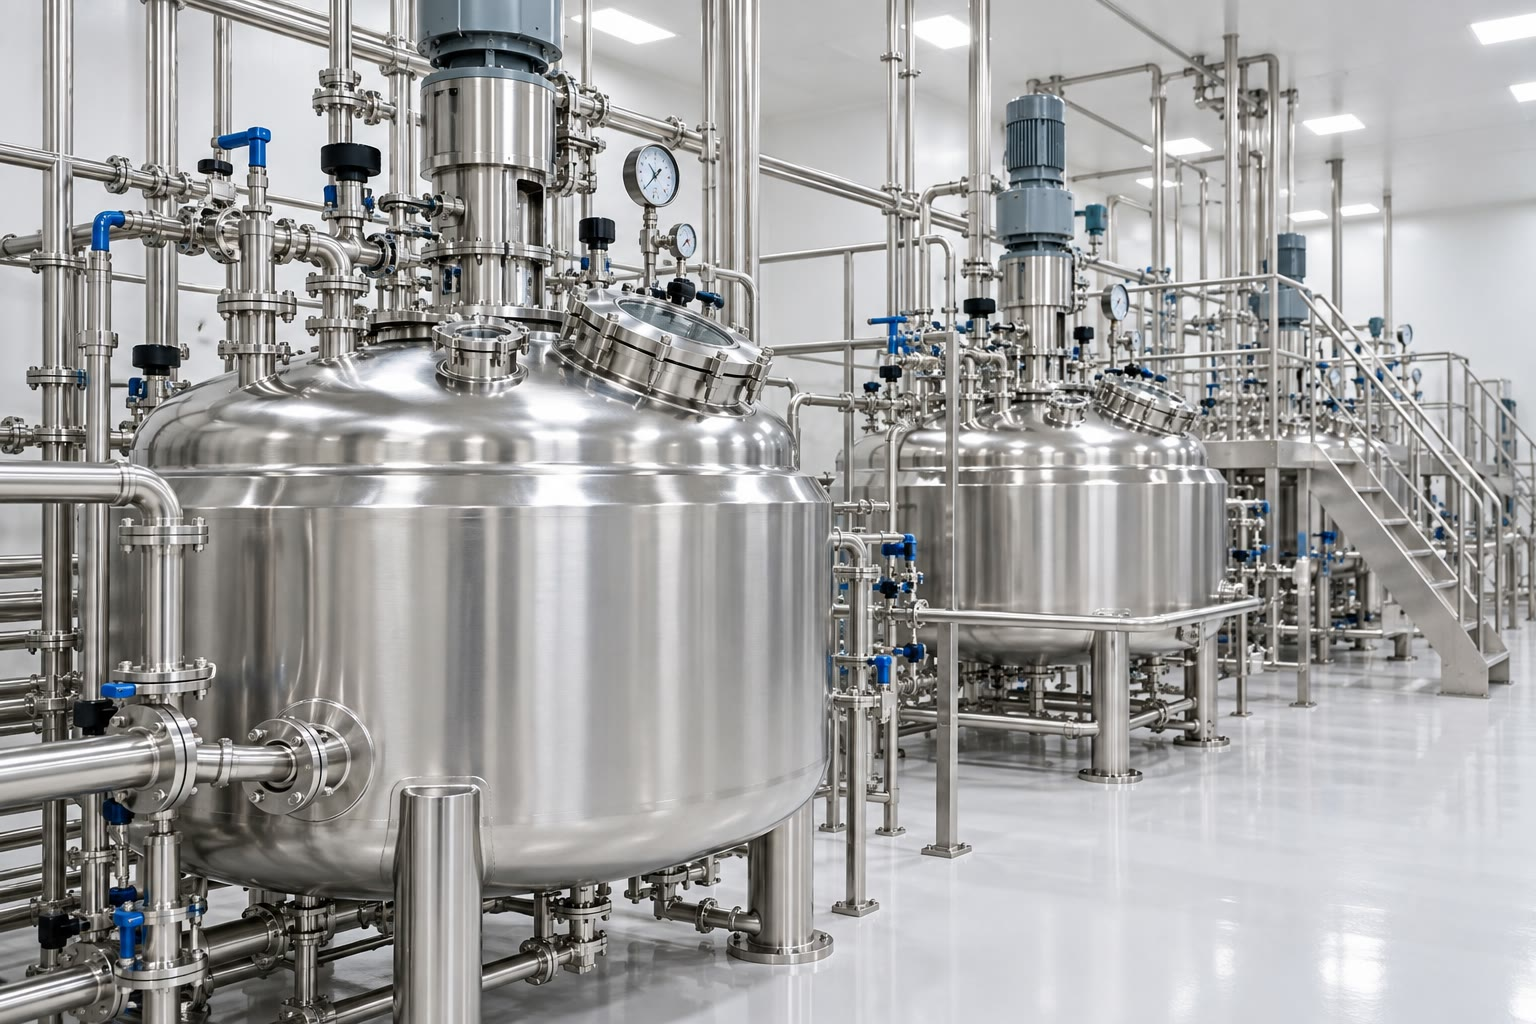
\includegraphics[width=0.55\linewidth]{images/book1/ai/g10-pharma-reactor.jpg}

{\small एक औषधि संयंत्र के स्टील रिएक्टर: प्रयोगशाला का एक \omterm{def:g10:synthesis-yield:synthesis}{संश्लेषण},
दस लाख गुना बड़ा।}
\end{omfigure}

\section{संश्लेषण के चरण}

\begin{definition}[संश्लेषण, अपरिष्कृत उत्पाद]\label{def:g10:synthesis-yield:synthesis}
\emph{संश्लेषण}\index{संश्लेषण} किसी \omterm{def:g6:pure-substances-and-mixtures:species}{रासायनिक स्पीशीज़} को दूसरी स्पीशीज़ से शुरू
करके, एक या कई \omterm{def:g7:chemical-reactions:reaction}{रासायनिक अभिक्रियाओं} द्वारा, तैयार करना है। किसी भी
शुद्धिकरण से पहले अभिक्रिया \omterm{def:g6:pure-substances-and-mixtures:mixture}{मिश्रण} से सीधे प्राप्त ठोस या द्रव
\emph{अपरिष्कृत उत्पाद}\index{अपरिष्कृत उत्पाद} है: उसमें अब भी \omterm{def:g7:chemical-reactions:reactant}{अभिकारक},
उपोत्पाद और \omterm{def:g6:solutions-and-solubility:solute}{विलायक} होते हैं।
\end{definition}

\begin{method}[संश्लेषण की योजना बनाना]\label{met:g10:synthesis-yield:plan}
\omterm{def:g10:synthesis-yield:synthesis}{संश्लेषण} चार चरणों में किया जाता है:
\begin{enumerate}
  \item \textbf{अभिक्रिया}: \omterm{def:g7:chemical-reactions:reactant}{अभिकारकों} को सही मात्राओं में मिलाइए, अक्सर
        उनमें से एक को आधिक्य में रखकर, और ज़रूरत हो तो गरम कीजिए।
  \item \textbf{पृथक्करण}: \omterm{def:g10:synthesis-yield:synthesis}{अपरिष्कृत उत्पाद} को अभिक्रिया \omterm{def:g6:pure-substances-and-mixtures:mixture}{मिश्रण} से अलग
        कीजिए (निस्यंदन, \omterm{def:g10:chemical-species:extraction}{निष्कर्षण})।
  \item \textbf{शुद्धिकरण}: \omterm{def:g10:synthesis-yield:synthesis}{अपरिष्कृत उत्पाद} से अशुद्धियाँ हटाइए
        (ठोस के लिए \omterm{def:g10:synthesis-yield:recrystallisation}{पुनःक्रिस्टलन}, द्रव के लिए \omterm{def:g10:chemical-species:distillation}{आसवन})।
  \item \textbf{विश्लेषण}: उत्पाद की पहचान और शुद्धता की जाँच कीजिए
        (गलनांक, वर्णलेखन), फिर उसे तौलिए और \omterm{def:g10:synthesis-yield:yield}{लब्धि}
        निकालिए।
\end{enumerate}
\end{method}

\begin{example}[ऐस्पिरिन बनाना]\label{ex:g10:synthesis-yield:aspirin}
सैलिसिलिक अम्ल एथेनोइक ऐनहाइड्राइड (जिसे ऐसीटिक ऐनहाइड्राइड भी कहते हैं) के
साथ अभिक्रिया करके ऐस्पिरिन और एथेनोइक अम्ल देता है:
\[
  \ce{C7H6O3 + C4H6O3 -> C9H8O4 + C2H4O2}
\]
\[
  \text{सैलिसिलिक अम्ल} + \text{एथेनोइक ऐनहाइड्राइड} \longrightarrow
  \text{ऐस्पिरिन} + \text{एथेनोइक अम्ल}.
\]
ऐनहाइड्राइड को आधिक्य में रखा जाता है, ताकि सारा सैलिसिलिक अम्ल अभिक्रिया करे;
बनने वाला एथेनोइक अम्ल एक उपोत्पाद है।
\end{example}

\begin{omfigure}
\setchemfig{atom sep=1.7em}
\begin{tabular}{@{}c@{\enspace}c@{\enspace}c@{\enspace}c@{\enspace}c@{\enspace}c@{\enspace}c@{}}
\chemfig{*6(-=-(-COOH)=(-OH)-=)} & $+$ &
\chemfig{H_3C-C(=[2]O)-O-C(=[2]O)-CH_3} & $\longrightarrow$ &
\chemfig{*6(-=-(-COOH)=(-O-[:150]C(=[:90]O)-[:210]H_3C)-=)} & $+$ &
\chemfig{H_3C-C(=[2]O)-OH} \\[2pt]
\small सैलिसिलिक अम्ल & & \small एथेनोइक ऐनहाइड्राइड & &
\small ऐस्पिरिन & & \small एथेनोइक अम्ल
\end{tabular}\par\medskip

{\small ऐस्पिरिन बनना, संरचना-सूत्रों में (षट्भुज का हर कोना एक कार्बन \omterm{def:g7:atoms-and-molecules:atom}{परमाणु} है,
जिस पर जहाँ कुछ और नहीं बना है वहाँ एक हाइड्रोजन \omterm{def:g7:atoms-and-molecules:atom}{परमाणु} है; आगे का एक अध्याय यह
संक्षिप्त रूप समझाता है)। सैलिसिलिक अम्ल की वलय पर लगा \ce{-OH}
समूह ऐनहाइड्राइड का आधा भाग ले लेता है; दूसरा आधा
एथेनोइक अम्ल के रूप में निकल जाता है।}
\end{omfigure}

\section{पश्चवाह तापन}

\begin{definition}[पश्चवाह तापन]\label{def:g10:synthesis-yield:reflux}
\emph{पश्चवाह तापन}\index{पश्चवाह तापन} किसी अभिक्रिया \omterm{def:g6:pure-substances-and-mixtures:mixture}{मिश्रण} को ऐसे फ़्लास्क में
गरम करना है जिसके ऊपर एक ऊर्ध्वाधर संघनित्र लगा हो: वाष्प ऊपर उठती है, संघनित्र
में ठंडी होती है, और द्रव वापस फ़्लास्क में बह आता है।
\end{definition}

\begin{proposition}[पश्चवाह क्यों]\label{prop:g10:synthesis-yield:why-reflux}
गरम करने से ज़्यादातर अभिक्रियाएँ तेज़ हो जाती हैं; पश्चवाह \omterm{def:g6:pure-substances-and-mixtures:mixture}{मिश्रण} के क्वथन ताप पर
जितनी देर ज़रूरत हो उतनी देर गरम करने देता है, और कोई \omterm{def:g7:chemical-reactions:reactant}{अभिकारक}, उत्पाद या \omterm{def:g6:solutions-and-solubility:solute}{विलायक}
वाष्प बनकर नहीं खोता।
\end{proposition}

\begin{proof}
उबलते द्रव का ताप उसके क्वथनांक से ऊपर नहीं जा सकता,
और द्रव से निकलने वाली हर वाष्प संघनित होकर लौट आती है:
उपकरण से कुछ नहीं निकलता, और वह ऊपर से खुला रहता है ताकि कोई
दाब न बने।
\end{proof}

\begin{omfigure}
\begin{tikzpicture}[font=\small, scale=1.05]
  \pic[transform shape] at (0,0) {heatingmantle};
  \pic[transform shape] at (0,0) {rbflask={0.42}{orange!25}};
  \foreach \p in {(-0.3,0.25), (0.2,0.18), (0.45,0.4), (-0.5,0.5)}
    \fill[black!45] \p circle (0.05);
  \pic[transform shape] at (0,3.0) {condenser};
  \draw[omDef, thick, <-] (0.8,3.825) -- (1.9,3.825) node[right] {पानी अंदर};
  \draw[omDef, thick, ->] (0.8,5.375) -- (1.9,5.375) node[right] {पानी बाहर};
  \draw[omProp, thick, <-] (-0.18,5.8) -- (-1.4,6.1) node[left] {खुला ऊपरी सिरा};
  \draw[omProp, thick, <-] (-0.45,1.2) -- (-2.0,1.6)
    node[left, align=right] {अभिक्रिया मिश्रण\\ और क्वथन-पत्थर};
  \draw[omProp, thick, <-] (-1.35,-0.2) -- (-2.0,-0.6)
    node[left] {तापन मैंटल};
  \draw[omThm, ->, thick] (-0.05,3.4) -- (-0.05,4.3);
  \draw[omDef, ->, thick] (0.05,4.3) -- (0.05,3.4);
  \node[omThm, anchor=east, font=\footnotesize] at (-0.45,4.6) {वाष्प उठती है};
  \node[omDef, anchor=west, font=\footnotesize] at (0.85,4.6) {द्रव वापस गिरता है};
\end{tikzpicture}

{\small \omterm{def:g10:synthesis-yield:reflux}{पश्चवाह तापन}। ठंडा पानी संघनित्र के आवरण में नीचे से प्रवेश करता है और
ऊपर से निकलता है, ताकि आवरण हमेशा
भरा रहे।}
\end{omfigure}

\begin{remark}[पानी नीचे से अंदर]\label{rem:g10:synthesis-yield:water}
ऊपर से डाला जाए, तो पानी सीधे नीचे बह जाएगा और आवरण का ऊपरी भाग \omterm{def:g4:air-a-mixture-of-gases:air}{वायु} से भरा
रहेगा; नीचे से डाला जाए, तो उसे निकलने से पहले पूरा आवरण
भरना पड़ता है।
\end{remark}

\section{पृथक्करण और शुद्धिकरण}

\begin{definition}[निर्वात निस्यंदन]\label{def:g10:synthesis-yield:vacuum-filtration}
\emph{निर्वात निस्यंदन}\index{निर्वात निस्यंदन} ऐसा निस्यंदन है जिसमें द्रव को
चूषण द्वारा फ़िल्टर पेपर से खींचा जाता है: छिद्रित प्लेट वाली एक चपटी
कीप (ब्यूख़नर कीप) एक साइड-आर्म फ़्लास्क पर बैठी होती है, जो एक निर्वात पंप से
जुड़ा होता है।
\end{definition}

\begin{omfigure}
\begin{tikzpicture}[font=\small, scale=1.05]
  \pic[transform shape] (ff) at (0,0) {filterflask={0.12}{orange!20}};
  \fill[black!50] (-0.3,2.45) rectangle (0.3,2.8);
  \pic[transform shape] at (0,2.45) {buchner={black!8}};
  \draw[black!60, line width=2pt] (ff-arm) -- (2.6,2.2);
  \draw[omProp, thick, ->] (2.7,2.2) -- (3.4,2.2) node[right,
    align=left, text=black] {निर्वात\\ पंप की ओर};
  \draw[omProp, thick, <-] (0.7,3.8) -- (1.9,4.3) node[right, text=black]
    {फ़िल्टर पेपर पर क्रिस्टल};
  \draw[omProp, thick, <-] (-0.4,0.15) -- (-1.8,0.6) node[left, text=black]
    {निस्यंद};
  \draw[omProp, thick, <-] (-0.3,2.6) -- (-1.8,2.9) node[left, text=black]
    {रबर की सील};
\end{tikzpicture}

{\small ब्यूख़नर कीप से \omterm{def:g10:synthesis-yield:vacuum-filtration}{निर्वात निस्यंदन}: पंप द्रव को जल्दी खींच लेता है और
ठोस को लगभग सूखा छोड़ देता है।}
\end{omfigure}

\begin{definition}[पुनःक्रिस्टलन]\label{def:g10:synthesis-yield:recrystallisation}
\emph{पुनःक्रिस्टलन}\index{पुनःक्रिस्टलन} किसी ठोस को गरम \omterm{def:g6:solutions-and-solubility:solute}{विलायक} के सबसे कम
संभव आयतन में घोलकर, फिर विलयन को ठंडा होने देकर, शुद्ध करता है: उत्पाद, जो ठंडे
में कहीं कम \omterm{def:g6:solutions-and-solubility:solute}{विलेय} है, क्रिस्टल बनकर निकल आता है, जबकि अशुद्धियाँ, जो थोड़ी मात्रा
में हैं, घुली रहती हैं।
\end{definition}

\begin{method}[किसी ठोस का पुनःक्रिस्टलन]\label{met:g10:synthesis-yield:recrystallise}
\begin{enumerate}
  \item ऐसा \omterm{def:g6:solutions-and-solubility:solute}{विलायक} चुनिए जिसमें उत्पाद गरम होने पर बहुत \omterm{def:g6:solutions-and-solubility:solute}{विलेय} हो और ठंडा होने
        पर लगभग अविलेय।
  \item अपरिष्कृत ठोस में गरम \omterm{def:g6:solutions-and-solubility:solute}{विलायक} थोड़ा-थोड़ा करके डालिए, ठीक तब तक
        जब तक वह पूरा घुल न जाए।
  \item विलयन को धीरे-धीरे ठंडा होने दीजिए, फिर बर्फ़-स्नान में: क्रिस्टल
        बनते हैं।
  \item उन्हें \omterm{def:g10:synthesis-yield:vacuum-filtration}{निर्वात निस्यंदन} से इकट्ठा कीजिए, थोड़े-से बर्फ़-ठंडे \omterm{def:g6:solutions-and-solubility:solute}{विलायक} से
        धोइए, और सुखाइए।
\end{enumerate}
\end{method}


\begin{omfigure}
\begin{tikzpicture}[font=\small]
  % 1. crude solid + a little hot solvent, on a hot plate
  \pic at (0,0.3) {hotplate};
  \pic at (0,0.3) {erlenmeyer={0.18}{orange!12}};
  \foreach \p in {(-0.4,0.42),(-0.15,0.38),(0.1,0.45),(0.35,0.4),(-0.3,0.55),(0.2,0.6)}
    \fill[brown!60] \p circle (0.06);
  \node[align=center, anchor=north] at (0,-0.15) {1. अपरिष्कृत ठोस,\\ गरम विलायक};
  % 2. clear hot solution
  \pic at (3,0.3) {hotplate};
  \pic at (3,0.3) {erlenmeyer={0.22}{orange!12}};
  \node[align=center, anchor=north] at (3,-0.15) {2. सब घुला,\\ स्वच्छ और गरम};
  % 3. ice bath: crystals
  \fill[cyan!12, draw=black!40] (5.0,0) rectangle (7.0,1.2);
  \foreach \p in {(5.2,0.9),(6.75,1.0),(5.3,0.3),(6.8,0.25)}
    \draw[black!35, fill=white] \p ++(-0.12,-0.1) rectangle ++(0.24,0.2);
  \pic at (6,0.1) {erlenmeyer={0.2}{orange!8}};
  \foreach \x/\y in {-0.45/0.18,-0.25/0.15,0/0.2,0.25/0.15,0.45/0.2,-0.1/0.3,0.15/0.32,
                     -0.35/0.32,0.35/0.33}
    \fill[white, draw=black!55] (6+\x,0.1+\y) -- ++(0.07,0.06) -- ++(0.07,-0.06)
      -- ++(-0.07,-0.06) -- cycle;
  \node[align=center, anchor=north] at (6,-0.15) {3. बर्फ़ में ठंडा करें:\\ क्रिस्टल बनते हैं};
  % 4. filter
  \pic at (9,0) {filterflask={0.12}{orange!12}};
  \pic at (9,2.45) {buchner={black!12}};
  \fill[black!50] (8.7,2.45) rectangle (9.3,2.8);
  \node[align=center, anchor=north] at (9,-0.15) {4. निर्वात निस्यंदन,\\ ठंडे से धोएँ, सुखाएँ};
\end{tikzpicture}

{\small चार चरणों में \omterm{def:g10:synthesis-yield:recrystallisation}{पुनःक्रिस्टलन}। अशुद्धियाँ ठंडे \omterm{def:g6:solutions-and-solubility:solute}{विलायक} में घुली रहती हैं और
\omterm{def:g3:separating-mixtures:filter}{निस्यंद} में चली जाती हैं।}
\end{omfigure}

\begin{remark}[हानि से बचा नहीं जा सकता]\label{rem:g10:synthesis-yield:losses}
% ledger: sol:aspirin-25, sol:aspirin-37
ठंडा होने पर भी \omterm{def:g6:solutions-and-solubility:solute}{विलायक} कुछ उत्पाद घुला हुआ रखता है। ऐस्पिरिन पानी में
\qty{25}{\celsius} पर लगभग \qty{3.3}{g/L} \omterm{def:g2:mixing-and-dissolving:dissolve}{घुलती} है, \qty{37}{\celsius} पर तीन
गुना अधिक, और और गरम होने पर कहीं अधिक: \omterm{def:g3:separating-mixtures:filter}{निस्यंद} और धोने के पानी का हर मिलीलीटर
थोड़ी-सी ऐस्पिरिन बहा ले जाता है। \omterm{def:g10:synthesis-yield:recrystallisation}{पुनःक्रिस्टलन} द्रव्यमान की क़ीमत पर शुद्धता
ख़रीदता है।
\end{remark}

\section{उत्पाद का विश्लेषण}

\begin{proposition}[शुद्धता की दो जाँचें]\label{prop:g10:synthesis-yield:checks}
संश्लेषित ठोस, इन परीक्षणों की सीमाओं के भीतर, शुद्ध है जब:
\begin{itemize}
  \item वह सारणियों में दिए गलनांक पर तीक्ष्णता से पिघलता है;
  \item \omterm{def:g10:chemical-species:tlc}{पतली परत वर्णलेखन} प्लेट पर वह एक ही धब्बा देता है,
        \omterm{def:g6:pure-substances-and-mixtures:pure-substance}{शुद्ध पदार्थ} के नमूने जितनी ऊँचाई पर।
\end{itemize}
\end{proposition}

\begin{proof}
स्वीकृत: अशुद्धि गलनांक को घटाती है और उसे एक परास में फैला देती है
(\cref{ch:g10:chemical-species}), और कोई दूसरी स्पीशीज़ आम तौर पर प्लेट पर
अलग दूरी तय करती है।
\end{proof}

\begin{omfigure}
\begin{tikzpicture}[font=\small, scale=1.3]
  \pic[transform shape] at (0,0) {tlcplate};
  \draw[black!50, dashed] (-0.7,2.7) -- (0.7,2.7);
  % lanes: C crude, R recrystallised, A aspirin, S salicylic acid
  \foreach \x/\l in {-0.5/C,-0.17/R,0.17/A,0.5/S}
    \node[font=\footnotesize, anchor=north] at (\x,0.38) {\l};
  \fill[omDef!70] (-0.5,1.75) ellipse (0.09 and 0.06);
  \fill[omDef!40] (-0.5,1.25) ellipse (0.09 and 0.06);
  \fill[omDef!70] (-0.17,1.75) ellipse (0.09 and 0.06);
  \fill[omDef!70] (0.17,1.75) ellipse (0.09 and 0.06);
  \fill[omDef!70] (0.5,1.25) ellipse (0.09 and 0.06);
  \node[anchor=west, font=\footnotesize] at (0.85,2.7) {विलायक अग्र};
  \node[anchor=west, font=\footnotesize] at (0.85,0.4) {प्रारंभ-रेखा};
\end{tikzpicture}

{\small शुद्ध ऐस्पिरिन (A) और सैलिसिलिक अम्ल (S) के बगल में \omterm{def:g10:synthesis-yield:synthesis}{अपरिष्कृत उत्पाद} (C) और
पुनःक्रिस्टलित उत्पाद (R) का वर्णलेखन, पराबैंगनी प्रकाश में। \omterm{def:g10:synthesis-yield:synthesis}{अपरिष्कृत
उत्पाद} में अब भी सैलिसिलिक अम्ल है; पुनःक्रिस्टलित
में नहीं।}
\end{omfigure}

\section{लब्धि}

\begin{definition}[लब्धि]\label{def:g10:synthesis-yield:yield}
किसी \omterm{def:g10:synthesis-yield:synthesis}{संश्लेषण} की \emph{लब्धि}\index{लब्धि} $\eta$ वास्तव में प्राप्त, शुद्ध और
सूखे, उत्पाद की मात्रा और \omterm{def:g10:reaction-progress-table:limiting}{सीमांत अभिकारक} से मिल सकने वाली अधिकतम मात्रा का
अनुपात है:
\[
  \eta = \frac{n_{\text{प्राप्त}}}{n_{\max}} ,
\]
जिसे आम तौर पर प्रतिशत में दिया जाता है।
\end{definition}

\begin{proposition}[द्रव्यमानों से लब्धि]\label{prop:g10:synthesis-yield:masses}
चूँकि प्राप्त और अधिकतम मात्राएँ एक ही उत्पाद की हैं, जिसका \omterm{def:g10:the-mole:molar-mass}{मोलर
द्रव्यमान} $M$ है, \omterm{def:g10:synthesis-yield:yield}{लब्धि} द्रव्यमानों का अनुपात भी है:
\[
  \eta = \frac{m_{\text{प्राप्त}}}{m_{\max}},
  \qquad m_{\max} = n_{\max} \times M,
\]
जहाँ $n_{\max}$ \omterm{def:g10:reaction-progress-table:extent}{प्रगति सारणी} से, $x = x_{\max}$ पर, आता है।
\end{proposition}

\begin{proof}
$m_{\text{प्राप्त}} / m_{\max} = (n_{\text{प्राप्त}} M) / (n_{\max} M)
= n_{\text{प्राप्त}} / n_{\max}$।
\end{proof}

\begin{example}[एक छोटे संश्लेषण की लब्धि]\label{ex:g10:synthesis-yield:small}
% ledger: aw:C, aw:H, aw:O
\qty{1.38}{g} सैलिसिलिक अम्ल ($M = \qty{138.0}{g/mol}$), यानी
\qty{0.0100}{mol}, आधिक्य एथेनोइक ऐनहाइड्राइड के साथ अभिक्रिया करता है। ऐस्पिरिन की
अधिकतम मात्रा \qty{0.0100}{mol} है, यानी
$0.0100 \times 180.0 = \qty{1.80}{g}$। अगर \qty{1.35}{g} शुद्ध सूखी
ऐस्पिरिन मिलती है, तो $\eta = 1.35 / 1.80 = 0.75$, यानी
\qty{75}{\percent} की \omterm{def:g10:synthesis-yield:yield}{लब्धि}।
\end{example}

\begin{remark}[लब्धि 100 \% से कम क्यों होती है]\label{rem:g10:synthesis-yield:below}
हर चरण में उत्पाद खोता है: काँच के उपकरणों पर चिपककर, \omterm{def:g3:separating-mixtures:filter}{निस्यंद} और धोने के पानी में
घुलकर, \omterm{def:g10:synthesis-yield:recrystallisation}{पुनःक्रिस्टलन} में पीछे छूटकर; कुछ अभिक्रियाएँ उपोत्पाद भी देती हैं, या \omterm{def:g10:reaction-progress-table:limiting}{सीमांत
अभिकारक} के खपने से पहले रुक जाती हैं। \qty{100}{\percent} से अधिक \omterm{def:g10:synthesis-yield:yield}{लब्धि} हमेशा किसी
त्रुटि का संकेत है, ज़्यादातर ऐसे उत्पाद का जिसे गीला या अशुद्ध रहते
तौल लिया गया।
\end{remark}

\begin{inthelab}[ऐस्पिरिन बनाना]
एक सूखे फ़्लास्क में शिक्षक सैलिसिलिक अम्ल को आधिक्य एथेनोइक ऐनहाइड्राइड और
अभिक्रिया को तेज़ करने वाले एक अम्ल की कुछ बूँदों के साथ मिलाते हैं, और \omterm{def:g6:pure-substances-and-mixtures:mixture}{मिश्रण} को
लगभग \qty{80}{\celsius} के जल-स्नान में पंद्रह मिनट तक पश्चवाह के साथ गरम करते हैं।
ठंडा होने के बाद ठंडा पानी मिलाया जाता है: आधिक्य ऐनहाइड्राइड उसके साथ अभिक्रिया
करता है, और ऐस्पिरिन, जो ठंडे पानी में मुश्किल से \omterm{def:g2:mixing-and-dissolving:dissolve}{घुलती} है, सफ़ेद क्रिस्टलों के रूप में
निकल आती है। इन्हें \omterm{def:g10:synthesis-yield:vacuum-filtration}{निर्वात निस्यंदन} से इकट्ठा किया जाता है, पुनःक्रिस्टलित किया
जाता है, सुखाया जाता है, तौला जाता है, और उनका गलनांक
मापा जाता है।
\end{inthelab}

\begin{safety}{\ghs[0.82cm]{GHS02}\ghs[0.82cm]{GHS05}\ghs[0.82cm]{GHS06}\ghs[0.82cm]{GHS07}}
% ledger: ghs:acetic-anhydride, ghs:salicylic, ghs:aspirin
एथेनोइक ऐनहाइड्राइड ज्वलनशील है, निगलने या साँस में लेने पर हानिकारक है, और त्वचा और
आँखों को गंभीर रूप से जलाता है: इसे शिक्षक धूम-हुड के नीचे,
दस्ताने और चश्मा पहनकर, सँभालते हैं। सैलिसिलिक अम्ल निगलने पर हानिकारक है और
आँखों को हानि पहुँचा सकता है। प्रयोगशाला में बनी ऐस्पिरिन कभी
दवा के रूप में नहीं ली जाती।
\end{safety}

\begin{omfigure}
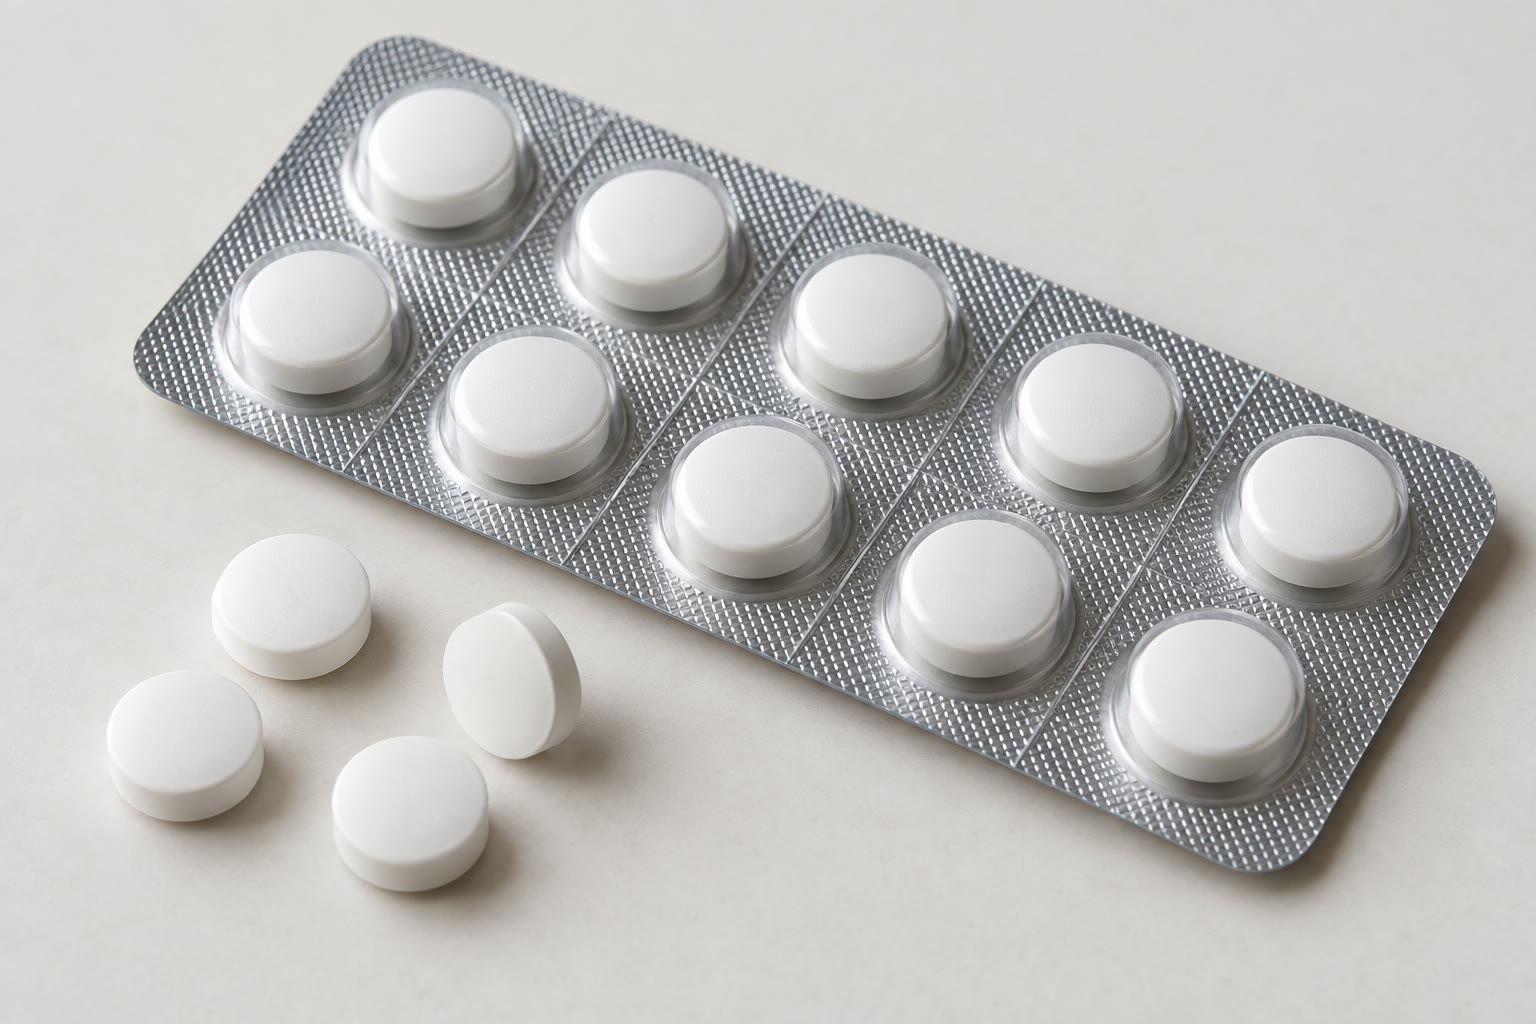
\includegraphics[width=0.45\linewidth]{images/book1/ai/g10-aspirin-tablets.jpg}

{\small ऐस्पिरिन की गोलियाँ: हर एक में \omterm{def:g6:pure-substances-and-mixtures:pure-substance}{शुद्ध पदार्थ} का एक तौला हुआ द्रव्यमान है,
एक बंधक के साथ मिला हुआ।}
\end{omfigure}

\section{अभ्यास}


\begin{exercise}[$\star$]\label{exo:g10:synthesis-yield:1}
एक \omterm{def:g10:synthesis-yield:synthesis}{संश्लेषण} अधिक से अधिक \qty{5.0}{g} उत्पाद दे सकता था; \qty{4.2}{g}
शुद्ध सूखा उत्पाद मिलता है। \omterm{def:g10:synthesis-yield:yield}{लब्धि} निकालिए।
\end{exercise}

\begin{exercise}[$\star$]\label{exo:g10:synthesis-yield:2}
किसी \omterm{def:g10:synthesis-yield:synthesis}{संश्लेषण} के इन चरणों को क्रम में लगाइए: गलनांक मापना;
\omterm{def:g10:synthesis-yield:reflux}{पश्चवाह तापन}; \omterm{def:g10:synthesis-yield:recrystallisation}{पुनःक्रिस्टलन}; \omterm{def:g10:synthesis-yield:synthesis}{अपरिष्कृत उत्पाद} का \omterm{def:g10:synthesis-yield:vacuum-filtration}{निर्वात
निस्यंदन}; \omterm{def:g7:chemical-reactions:reactant}{अभिकारकों} को तौलना।
\end{exercise}

\begin{exercise}[$\star$]\label{exo:g10:synthesis-yield:3}
पश्चवाह व्यवस्था में ठंडा करने वाला पानी संघनित्र में नीचे से क्यों डाला जाता है?
संघनित्र का ऊपरी सिरा खुला क्यों छोड़ा जाता है?
\end{exercise}

\begin{exercise}[$\star$]\label{exo:g10:synthesis-yield:4}
किसी उत्पाद के \omterm{def:g10:synthesis-yield:recrystallisation}{पुनःक्रिस्टलन} के लिए \omterm{def:g6:solutions-and-solubility:solute}{विलायक} में कौन-से दो गुण होने चाहिए?
अशुद्धियाँ कहाँ पहुँचती हैं?
\end{exercise}

\begin{exercise}[$\star$]\label{exo:g10:synthesis-yield:5}
% ledger: mp:aspirin
संश्लेषित ऐस्पिरिन का एक नमूना \qty{124}{\celsius} और
\qty{130}{\celsius} के बीच पिघलता है। शुद्ध ऐस्पिरिन लगभग \qty{135}{\celsius} पर
पिघलती है। क्या नमूना शुद्ध है? क्या करना चाहिए?
\end{exercise}

\begin{exercise}[$\star\star$]\label{exo:g10:synthesis-yield:6}
\qty{2.00}{g} सैलिसिलिक अम्ल आधिक्य एथेनोइक ऐनहाइड्राइड के साथ अभिक्रिया करता है;
\qty{2.03}{g} शुद्ध सूखी ऐस्पिरिन मिलती है। ऐस्पिरिन का अधिकतम द्रव्यमान
और \omterm{def:g10:synthesis-yield:yield}{लब्धि} निकालिए।
\end{exercise}

\begin{exercise}[$\star\star$]\label{exo:g10:synthesis-yield:7}
एक छात्रा अपनी ऐस्पिरिन को गीली रहते ही तौल लेती है और
\qty{104}{\percent} \omterm{def:g10:synthesis-yield:yield}{लब्धि} पाती है। समझाइए। अगर \omterm{def:g10:synthesis-yield:synthesis}{अपरिष्कृत उत्पाद} को, बिना शुद्ध
किए पर सूखा, तौला जाए, तो \omterm{def:g10:synthesis-yield:yield}{लब्धि} वास्तविक \omterm{def:g10:synthesis-yield:yield}{लब्धि} की तुलना में बहुत अधिक आएगी या
बहुत कम?
\end{exercise}

\begin{exercise}[$\star\star$]\label{exo:g10:synthesis-yield:8}
क्रिस्टल इकट्ठा करने के लिए कागज़ के शंकु से साधारण निस्यंदन की तुलना में \omterm{def:g10:synthesis-yield:vacuum-filtration}{निर्वात
निस्यंदन} के दो लाभ बताइए।
\end{exercise}

\begin{exercise}[$\star\star$]\label{exo:g10:synthesis-yield:9}
एक वर्णलेखन प्लेट पर \omterm{def:g6:solutions-and-solubility:solute}{विलायक} अग्र \qty{5.0}{cm} आगे बढ़ा है। एक
संश्लेषित उत्पाद का धब्बा \qty{3.1}{cm} बढ़ा है, शुद्ध
ऐस्पिरिन का \qty{3.1}{cm}, सैलिसिलिक अम्ल का \qty{2.2}{cm}। तीनों
\omterm{def:g10:chemical-species:retention-factor}{मंदन गुणांक} निकालिए। उत्पाद के बारे में क्या निष्कर्ष निकाला जा सकता है?
\end{exercise}

\begin{exercise}[$\star\star$]\label{exo:g10:synthesis-yield:10}
दो \omterm{def:g6:solutions-and-solubility:solute}{विलायकों} में किसी उत्पाद की \omterm{def:g6:solutions-and-solubility:solubility}{विलेयता} है:
\begin{center}
\begin{tabular}{lcc}
\hline
\omterm{def:g6:solutions-and-solubility:solute}{विलायक} & ठंडा (\qty{20}{\celsius}) & गरम (क्वथन के पास) \\
\hline
A & \qty{2}{g/L} & \qty{150}{g/L} \\
B & \qty{80}{g/L} & \qty{120}{g/L} \\
\hline
\end{tabular}
\end{center}
\omterm{def:g10:synthesis-yield:recrystallisation}{पुनःक्रिस्टलन} के लिए कौन-सा \omterm{def:g6:solutions-and-solubility:solute}{विलायक} बेहतर है? \qty{3.0}{g} \omterm{def:g10:synthesis-yield:synthesis}{अपरिष्कृत
उत्पाद} के लिए लगभग कितना गरम \omterm{def:g6:solutions-and-solubility:solute}{विलायक} चाहिए, और ठंडा होने पर अधिक से अधिक कितना
द्रव्यमान घुला रहता है?
\end{exercise}

\begin{exercise}[$\star\star$]\label{exo:g10:synthesis-yield:11}
पश्चवाह व्यवस्था का गोल पेंदी वाला फ़्लास्क कभी आधे से अधिक क्यों नहीं भरा जाता?
क्वथन-पत्थर क्यों डाले जाते हैं?
\end{exercise}

\begin{exercise}[$\star\star\star$]\label{exo:g10:synthesis-yield:12}
एक दवा दो चरणों में बनाई जाती है, जिनकी \omterm{def:g10:synthesis-yield:yield}{लब्धियाँ} \qty{80}{\percent} और
\qty{70}{\percent} हैं। समग्र \omterm{def:g10:synthesis-yield:yield}{लब्धि} क्या है? \qty{90}{\percent} वाले तीन चरणों
के लिए वह क्या होगी? रसायनज्ञ दवाओं को यथासंभव कम चरणों में बनाने की कोशिश क्यों
करते हैं?
\end{exercise}

\begin{exercise}[$\star\star\star$]\label{exo:g10:synthesis-yield:13}
% ledger: sol:aspirin-25
ऐस्पिरिन पानी में \qty{25}{\celsius} पर लगभग \qty{3.3}{g/L}
\omterm{def:g2:mixing-and-dissolving:dissolve}{घुलती} है। क्रिस्टलों को उस ताप पर \qty{50}{mL} पानी से धोया जाता है।
अधिक से अधिक कितनी ऐस्पिरिन खो सकती है? धोने का पानी पहले बर्फ़ में ठंडा क्यों किया
जाता है?
\end{exercise}

\begin{exercise}[$\star\star\star$]\label{exo:g10:synthesis-yield:14}
\qty{2.76}{g} सैलिसिलिक अम्ल को \qty{0.0500}{mol}
एथेनोइक ऐनहाइड्राइड के साथ मिलाया जाता है। अभिक्रिया के बाद पानी मिलाया जाता है,
जो आधिक्य ऐनहाइड्राइड को नष्ट कर देता है: \ce{C4H6O3 + H2O -> 2C2H4O2}।
\begin{enumerate}
  \item \omterm{def:g10:synthesis-yield:synthesis}{संश्लेषण} की \omterm{def:g10:reaction-progress-table:extent}{प्रगति सारणी} भरिए; ऐनहाइड्राइड की कितनी
        मात्रा बचती है?
  \item अंत में एथेनोइक अम्ल की कुल कितनी मात्रा मौजूद है?
\end{enumerate}
\end{exercise}

\begin{exercise}[$\star\star\star$]\label{exo:g10:synthesis-yield:15}
एक कारख़ाने को सैलिसिलिक अम्ल से \qty{85}{\percent} की समग्र \omterm{def:g10:synthesis-yield:yield}{लब्धि} के साथ
\qty{1.00}{t} ऐस्पिरिन बनानी है। उसे सैलिसिलिक अम्ल का कितना द्रव्यमान
ख़रीदना होगा?
\end{exercise}

\section{समस्या: ऐस्पिरिन बनाना}

\begin{problem}[{सप्ताहांत समस्या --- तीन ग्राम सैलिसिलिक अम्ल से शुद्ध ऐस्पिरिन के
एक जार तक: लब्धि क्या है?}]
\label{pb:g10:synthesis-yield:1}
% ledger: rho:acetic-anhydride, mp:aspirin, mp:salicylic, sol:aspirin-25, aw:C, aw:H, aw:O
एक कक्षा ऐस्पिरिन बनाती है। फ़्लास्क में: \qty{3.0}{g} सैलिसिलिक अम्ल और
\qty{6.0}{mL} एथेनोइक ऐनहाइड्राइड, जिसका घनत्व \qty{1.08}{g/mL} है, साथ में
अम्ल की कुछ बूँदें; \omterm{def:g6:pure-substances-and-mixtures:mixture}{मिश्रण} को पश्चवाह के साथ गरम किया जाता है। \omterm{def:g10:synthesis-yield:vacuum-filtration}{निर्वात निस्यंदन}
से इकट्ठा किया गया \omterm{def:g10:synthesis-yield:synthesis}{अपरिष्कृत उत्पाद} गीला होने पर \qty{3.6}{g} और सूखने पर
\qty{3.3}{g} का है। \omterm{def:g10:synthesis-yield:recrystallisation}{पुनःक्रिस्टलन} और सुखाने के बाद \qty{2.7}{g} सफ़ेद
क्रिस्टल बचते हैं।

\medskip
\noindent\textbf{भाग I --- अभिक्रिया।}
\begin{enumerate}
  \item जाँचिए कि समीकरण
        \ce{C7H6O3 + C4H6O3 -> C9H8O4 + C2H4O2} संतुलित है।
  \item सैलिसिलिक अम्ल, एथेनोइक ऐनहाइड्राइड, ऐस्पिरिन और एथेनोइक अम्ल के
        \omterm{def:g10:the-mole:molar-mass}{मोलर द्रव्यमान} निकालिए।
  \item \omterm{def:g7:chemical-reactions:reactant}{अभिकारकों}, वांछित उत्पाद और उपोत्पाद के नाम बताइए।
  \item \omterm{def:g6:pure-substances-and-mixtures:mixture}{मिश्रण} को खुले फ़्लास्क के बजाय पश्चवाह के साथ क्यों गरम किया
        जाता है?
\end{enumerate}

\medskip
\noindent\textbf{भाग II --- अधिकतम द्रव्यमान।}
\begin{enumerate}[resume]
  \item सैलिसिलिक अम्ल की प्रारंभिक मात्रा निकालिए।
  \item एथेनोइक ऐनहाइड्राइड का द्रव्यमान, फिर मात्रा, निकालिए।
  \item \omterm{def:g10:reaction-progress-table:extent}{प्रगति सारणी} भरिए। कौन-सा \omterm{def:g7:chemical-reactions:reactant}{अभिकारक} सीमांत है?
        $x_{\max}$ बताइए।
  \item ऐस्पिरिन का अधिकतम द्रव्यमान निकालिए।
  \item सैलिसिलिक अम्ल के बजाय ऐनहाइड्राइड को आधिक्य में क्यों रखा
        जाता है?
\end{enumerate}

\medskip
\noindent\textbf{भाग III --- पृथक्करण और शुद्धिकरण।}
\begin{enumerate}[resume]
  \item \omterm{def:g10:synthesis-yield:yield}{लब्धि} निकालने में गीले द्रव्यमान, \qty{3.6}{g}, का उपयोग क्यों नहीं किया
        जा सकता?
  \item सूखे \omterm{def:g10:synthesis-yield:synthesis}{अपरिष्कृत उत्पाद} की \omterm{def:g10:synthesis-yield:yield}{लब्धि} निकालिए।
  \item \omterm{def:g10:synthesis-yield:recrystallisation}{पुनःक्रिस्टलन} से द्रव्यमान क्यों घटता है?
  \item क्रिस्टलों को \qty{25}{\celsius} पर \qty{30}{mL} पानी से धोया गया, जिसमें
        ऐस्पिरिन लगभग \qty{3.3}{g/L} \omterm{def:g2:mixing-and-dissolving:dissolve}{घुलती} है। इस तरह अधिक से अधिक कितना
        द्रव्यमान खो सकता था?
  \item शुद्ध उत्पाद की \omterm{def:g10:synthesis-yield:yield}{लब्धि} निकालिए।
\end{enumerate}

\medskip
\noindent\textbf{भाग IV --- उत्पाद की जाँच।}
\begin{enumerate}[resume]
  \item पुनःक्रिस्टलित क्रिस्टल \qty{135}{\celsius} पर तीक्ष्णता से पिघलते हैं।
        इससे क्या पता चलता है?
  \item \omterm{def:g10:synthesis-yield:synthesis}{अपरिष्कृत उत्पाद} \qty{120}{\celsius} और
        \qty{131}{\celsius} के बीच पिघला था। इससे क्या पता चलता है?
  \item वर्णलेखन प्लेट पर \omterm{def:g10:synthesis-yield:synthesis}{अपरिष्कृत उत्पाद} दो धब्बे देता है,
        एक शुद्ध ऐस्पिरिन की ऊँचाई पर और एक सैलिसिलिक अम्ल की ऊँचाई पर;
        पुनःक्रिस्टलित उत्पाद एक धब्बा देता है, ऐस्पिरिन की
        ऊँचाई पर। निष्कर्ष निकालिए।
  \item पुनःक्रिस्टलित उत्पाद का धब्बा \qty{3.1}{cm} और \omterm{def:g6:solutions-and-solubility:solute}{विलायक} अग्र
        \qty{5.0}{cm} आगे बढ़ा। उसका \omterm{def:g10:chemical-species:retention-factor}{मंदन गुणांक} निकालिए।
  \item अभिक्रिया और \omterm{def:g10:synthesis-yield:recrystallisation}{पुनःक्रिस्टलन} के बीच, काम के किस भाग में अधिक
        ऐस्पिरिन खोई?
  \item अंतिम उत्तर बताइए: \omterm{def:g10:synthesis-yield:synthesis}{संश्लेषण} की \omterm{def:g10:synthesis-yield:yield}{लब्धि} क्या है?
\end{enumerate}
\end{problem}
